See Fig. \ref{eq:myfig:solutions/1/30/}

\begin{figure}[!ht]
\centering
\resizebox{\columnwidth}{!}{


\tikzset{every picture/.style={line width=0.75pt}} %set default line width to 0.75pt        

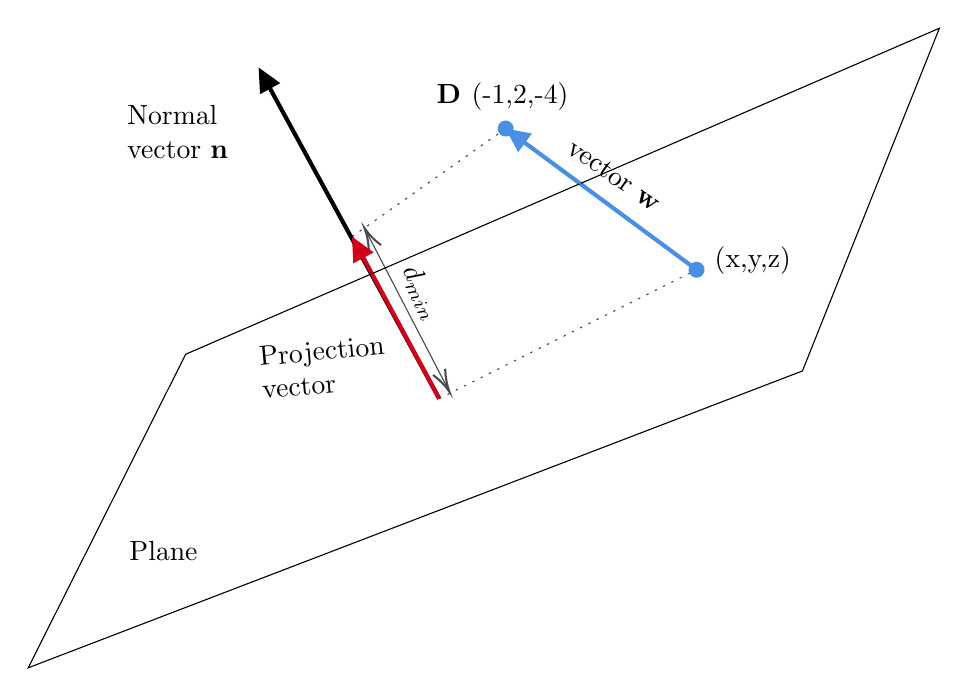
\begin{tikzpicture}[x=0.75pt,y=0.75pt,yscale=-1,xscale=1]
%uncomment if require: \path (0,324); %set diagram left start at 0, and has height of 324

%Straight Lines [id:da012474511036709712] 
\draw [color={rgb, 255:red, 74; green, 74; blue, 74 }  ,draw opacity=1 ] [dash pattern={on 0.84pt off 2.51pt}]  (165.51,108.36) -- (239.51,56.27) ;
%Straight Lines [id:da164610693713777] 
\draw [color={rgb, 255:red, 74; green, 74; blue, 74 }  ,draw opacity=1 ] [dash pattern={on 0.84pt off 2.51pt}]  (207.51,186.36) -- (331.51,124.27) ;
%Straight Lines [id:da0009900971082483778] 
\draw [color={rgb, 255:red, 74; green, 74; blue, 74 }  ,draw opacity=1 ]   (211.58,181.43) -- (172.42,105.98) ;
\draw [shift={(171.5,104.2)}, rotate = 422.57] [color={rgb, 255:red, 74; green, 74; blue, 74 }  ,draw opacity=1 ][line width=0.75]    (10.93,-3.29) .. controls (6.95,-1.4) and (3.31,-0.3) .. (0,0) .. controls (3.31,0.3) and (6.95,1.4) .. (10.93,3.29)   ;
\draw [shift={(212.5,183.2)}, rotate = 242.57] [color={rgb, 255:red, 74; green, 74; blue, 74 }  ,draw opacity=1 ][line width=0.75]    (10.93,-3.29) .. controls (6.95,-1.4) and (3.31,-0.3) .. (0,0) .. controls (3.31,0.3) and (6.95,1.4) .. (10.93,3.29)   ;
%Straight Lines [id:da6317108471264852] 
\draw [line width=1.5]    (207.51,186.36) -- (122.42,30.38) ;
\draw [shift={(120.51,26.87)}, rotate = 421.39] [fill={rgb, 255:red, 0; green, 0; blue, 0 }  ][line width=0.08]  [draw opacity=0] (11.61,-5.58) -- (0,0) -- (11.61,5.58) -- cycle    ;
%Straight Lines [id:da4711513779445873] 
\draw [color={rgb, 255:red, 74; green, 144; blue, 226 }  ,draw opacity=1 ][line width=1.5]    (331.51,124.27) -- (242.72,58.64) ;
\draw [shift={(239.51,56.27)}, rotate = 396.47] [fill={rgb, 255:red, 74; green, 144; blue, 226 }  ,fill opacity=1 ][line width=0.08]  [draw opacity=0] (11.61,-5.58) -- (0,0) -- (11.61,5.58) -- cycle    ;
%Straight Lines [id:da281513313013386] 
\draw [color={rgb, 255:red, 208; green, 2; blue, 27 }  ,draw opacity=1 ][line width=1.5]    (207.51,186.36) -- (167.4,111.89) ;
\draw [shift={(165.51,108.36)}, rotate = 421.7] [fill={rgb, 255:red, 208; green, 2; blue, 27 }  ,fill opacity=1 ][line width=0.08]  [draw opacity=0] (11.61,-5.58) -- (0,0) -- (11.61,5.58) -- cycle    ;
%Shape: Polygon [id:ds23253650680866844] 
\draw   (85.38,164.99) -- (448.5,7.93) -- (382.5,173.07) -- (9.5,316.07) -- (9.5,316.07) -- cycle ;
%Straight Lines [id:da02842289374539675] 
\draw [color={rgb, 255:red, 74; green, 144; blue, 226 }  ,draw opacity=1 ]   (239.51,56.27) -- (331.51,124.27) ;
\draw [shift={(331.51,124.27)}, rotate = 36.47] [color={rgb, 255:red, 74; green, 144; blue, 226 }  ,draw opacity=1 ][fill={rgb, 255:red, 74; green, 144; blue, 226 }  ,fill opacity=1 ][line width=0.75]      (0, 0) circle [x radius= 3.35, y radius= 3.35]   ;
\draw [shift={(239.51,56.27)}, rotate = 36.47] [color={rgb, 255:red, 74; green, 144; blue, 226 }  ,draw opacity=1 ][fill={rgb, 255:red, 74; green, 144; blue, 226 }  ,fill opacity=1 ][line width=0.75]      (0, 0) circle [x radius= 3.35, y radius= 3.35]   ;

% Text Node
\draw (56,44) node [anchor=north west][inner sep=0.75pt]   [align=left] {Normal \\vector \textbf{n} };
% Text Node
\draw (118.97,160.37) node [anchor=north west][inner sep=0.75pt]  [rotate=-354.79] [align=left] {Projection \\vector};
% Text Node
\draw (205,33) node [anchor=north west][inner sep=0.75pt]   [align=left] {\textbf{D }(-1,2,-4)};
% Text Node
\draw (339,112) node [anchor=north west][inner sep=0.75pt]   [align=left] {(x,y,z)};
% Text Node
\draw (272.66,59.12) node [anchor=north west][inner sep=0.75pt]  [rotate=-34.52] [align=left] {vector \textbf{w} };
% Text Node
\draw (198.69,119.24) node [anchor=north west][inner sep=0.75pt]  [rotate=-64.65] [align=left] {$d_{min}$};
% Text Node
\draw (57,254.07) node [anchor=north west][inner sep=0.75pt]   [align=left] {Plane};


\end{tikzpicture}
}
\caption{Isosceles Triangle with altitudes drawn to equal sides}
\label{eq:myfig:solutions/1/30/}
\end{figure}
 Let $\vec{m}_{AC}$ and $\vec{m}_{BE}$ be direction vector of side AC and altitude BE respectively.
 \begin{align}
 \vec{m}_{AC}=\vec{A-C}\\
 \vec{m}_{BE}=\vec{B-E}
 \end{align}
Here, BE  $\perp$ AC because BE is the altitude to side AC.So,
 \begin{align}
 \vec{m}_{AC}^{T}\vec{m}_{BE}=0\\
 \vec{(A-C)}^T\vec{(B-E)}=0\\
  \vec{(A-E+E-B+B-C)}^T\vec{(B-E)}=0\\
% \begin{multlined}
\vec{(A-E)}^T\vec{(B-E)}+\norm{\vec{B-E}}^2+\\ \vec{(B-C)}^T\vec{(B-E)}=0
\\
%\end{multlined}\\
\norm{\vec{B-E}}^2+\vec{(B-C)}^T\vec{(B-E)}=0 
\label{eq:solutions/1/30/2.0.7}
\end{align}
 Let $\vec{m}_{AB}$ and $\vec{m}_{CF}$ be direction vector of side AB and altitude CF respectively.
 \begin{align}
 \vec{m}_{AB}=\vec{A-B}\\
 \vec{m}_{CF}=\vec{C-F}
 \end{align}
 Here, CF  $\perp$ AB because CF is the altitude to side AB.So,
 \begin{align}
 \vec{m}_{AB}^T\vec{m}_{CF}=0\\
 \vec{(A-B)}^T\vec{(C-F)}=0\\
\vec{(A-F+F-C+C-B)}^T\vec{(C-F)}=0\\
%\begin{multlined}
 \vec{(A-F)}^T\vec{(C-F)}+\norm{\vec{C-F}}^2+\\ \vec{(C-B)}^T\vec{(C-F)}=0
\\
%\end{multlined}\\
\norm{\vec{C-F}}^2+\vec{(C-B)}^T\vec{(C-F)}=0\label{eq:solutions/1/30/2.0.14}
 \end{align}
 Comparing equation \eqref{eq:solutions/1/30/2.0.7} and \eqref{eq:solutions/1/30/2.0.14}
\begin{multline}
\norm{\vec{C-F}}^2+\vec{(C-B)}^T\vec{(C-F)}=\\\norm{\vec{B-E}}^2+\vec{(B-C)}^T\vec{(B-E)}
\end{multline}
\begin{multline}
\norm{\vec{C-F}}^2+\vec{(C-B)}^T\vec{(C-A+A-F)}=\\
\norm{\vec{B-E}}^2+\vec{(B-C)}^T\vec{(B-A+A-E)}
\end{multline}
\begin{multline}
\norm{\vec{C-F}}^2+\vec{(C-B)}^T\vec{(C-A)}+\vec{(C-B)}^T\vec{(A-F)}=\\
\norm{\vec{B-E}}^2+\vec{(B-C)}^T\vec{(B-A)}+\vec{(B-C)}^T\vec{(A-E)}
\end{multline}
\begin{multline}
\norm{\vec{C-F}}^2+2\vec{(C-B)}^T\vec{(C-A)}=\\
\norm{\vec{B-E}}^2+2\vec{(B-C)}^T\vec{(B-A)}
\end{multline}
\begin{multline}
\norm{\vec{C-F}}^2+2(\norm{\vec{C-B}}\norm{\vec{C-A}})\cos\theta=\\
\norm{\vec{B-E}}^2+2(\norm{\vec{B-C}}\norm{\vec{B-A}})\cos\theta
\end{multline}
\begin{align}
\norm{\vec{C-F}}^2=\norm{\vec{B-E}}^2\\
\norm{\vec{C-F}}=\norm{\vec{B-E}}
\end{align}
Hence, the altitudes drawn to equal sides of isosceles triangle is equal.
